\chapter{Sejarah Lingkungan}

\section{Lingkungan St. Theresia Kanak-kanak Yesus}
\begin{floatingfigure}[l]{2cm}
\begin{center}
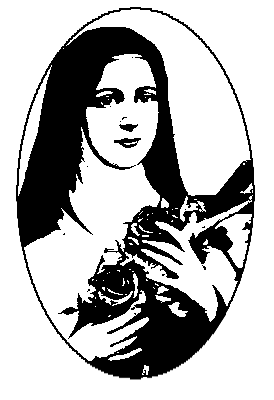
\includegraphics[scale=1]{theresia-logo.png}
\end{center}
\end{floatingfigure}
Lingkungan Santa Theresia Kanak-kanak Yesus adalah lingkungan baru di Stasi Bunda Maria Maguwo. Lingkungan ini merupakan hasil pemekaran dari lingkungan St. Petrus yang dirasa sudah terlalu banyak anggotanya. Lingkungan St. Petrus dimekarkan menjadi lingkungan St. Petrus, lingkungan St. Monika, dan lingkungan St. Theresia.

\color{black}
Pada akhir tahun 2013 yaitu pada bulan September, semua lingkungan di Stasi Maguwo 
diharapkan melakukan pemilihan pengurus baru. Sesuai dengan mekanisme pemilihan dari paroki, 
maka dilakukanlah pemilihan pengurus baru yang diketuai oleh Andreas Keso Muda.
Pemilihan berhasil memilih Anton Supriyana sebagai ketua baru. Beliau ini adalah warga baru namun stok lama. Beliau sudah lama berkecimpung di dewan paroki Pringwulung, tempat tinggal beliau sebelumnya.

Namun akhirnya lingkungan Petrus mekar menjadi 3 yaitu 
Lingkungan Petrus meliputi Kembang, Nanggulan, dan Tobong. Lingkungan St. Monica meliputi Maguwo, Sanggrahan, dan Karangnongko. Lingkungan ST. Theresia meliputi Pugeran dan Sombomerten. 

\subsection*{Umat St. Theresia}
Lingkungan St. Theresia mencakup \jumlahKlg{} keluarga dengan \jumlahLP{} umat dengan perincian \jumlahL{} laki-laki dan \jumlahP{} perempuan. Namun demikian ada beberapa mahasiswa yang terlibat aktif dalam kegiatan-kegiatan lingkungan dan tidak tercatat dengan pasti karena mobilitasnya yang tinggi.

\subsection*{Inventaris Peralatan Misa}
Sejak awal lahirnya lingkungan St. Theresia, umat sudah berkomitmen agar lingkungan mempunyai peralatan misa. Beberapa upaya yang dilakukan adalah pengumpulan data melalui tabungan receh, sumbangan sukarela, dan juga donatur dari luar. Puji syukur kepada Allah bahwa usaha-usaha tersebut banyak membuahkan hasil. Donatur dari luar, berkat ketekunan dari Bapak KRA YP Sunaryo Prononagoro lingkungan St. Theresia mendapat banyak peralatan misa. 
Peralatan misa yang dimiliki lingkungan antara lain:
\begin{itemize}
\item peralatan altar: salib kuningan dan kayu,
korporal,
purivicatorium,
taplak,
piala,
sibori,
piksis,
patena,
aspergil,
wirug,
krincingan,
tempat lilin besar \& kecil,
patung Bunda Maria,
nampan, ampul,
tempat minyak suci.
\item pakaian liturgi: kasula,
stola,
superpli,
gaun,
kerah lebar,
singel,
alba,
samir
\item buku:  TPE,
Liturgi Orang Sakit,
Mazmur Tanggapan, Sakramen Pemberkatan,
Aneka Ibadat Kristiani, teks doa rosario,
Puji Syukur, teks doa rosario bahasa Jawa.
\item elektronik: HT, \textit{wireless microphone \& speaker}, LCD projector.
\end{itemize} 

Perlu diketahui bahwa patung Bunda Maria Lourdes yang besar adalah sumbangan dari Bapak KRA YP Sunaryo Prononagoro.


\section{Riwayat St. Theresia Kanak-kanak Yesus}
Santa Theresia dari kanak-kanak Yesus dilahirkan di Alemon Perancis pada tgl 2 Januari 1873 dengan nama Maria Francoise Therese Martin. Ia berasal dari sebuah keluarga Katolik yang saleh, pasangan suami isteri Louis Martin dan Azelie Guerin. Ibunya meninggal waktu Theresia masih anak-anak. Sepeninggal ibu Theresia sangat terguncang sehingga Pauline kakaknya terpaksa menggantikan peran ibunya untuk merawat dan memperhatikan perkembangan Theresia.

\begin{floatingfigure}[l]{2.75cm}
\begin{center}
\includegraphics[scale=0.5]{theresia-1.jpg}
\end{center}
\end{floatingfigure}
Theresia sangat disayang oleh ayahnya dan mendapat berbagai julukan seperti "Theresia kecil" atau "Ratu Kecil" dsb. Tahun 1881 sampai 1885 Theresia bersekolah di sekolah suster-suster Benedictin, ia tumbuh menjadi seorang gadis kecil yang sangat perasa dan cepat menangis sehingga kurang akrab dengan teman-teman sekolahnya. Sifat perasanya semakin menjadi-jadi ketika Pauline kakak perempuannya masuk biara Carmel di Lisieux tahun 1882. Theresia jatuh sakit karena keberangkatan kakaknya itu, namun ia disembuhkan secara ajaib saat kakak-kakaknya berlutut dan berdoa disamping tempat tidur untuk kesembuhannya, penyakitnya hilang seketika meskipun sifat perasanya masih ada. Sifat perasa itu baru hilang setelah dinasihati oleh ayahnya pada perayaan Natal 1886, semenjak itu ia sadar akan sifat buruknya yang manja dan mudah tersinggung itu. Ia sadar bahwa sifat yang kekanak-kanakan itu sudah tidak cocok lagi bagi seorang remaja puteri yang bercita-cita menjadi suster.

\begin{floatingfigure}[r]{3.75cm}
\begin{center}
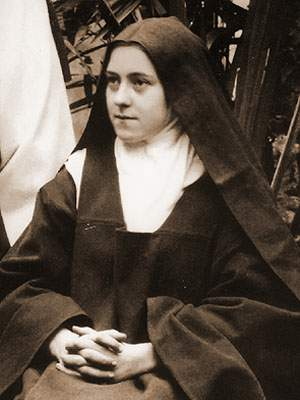
\includegraphics[scale=0.35]{theresia-2.jpg}
\end{center}
\end{floatingfigure}
Dalam autobiografinya, Theresia menyebutkan bahwa kesadaran ini mengawali kehidupannya yang baru, dimana Yesus telah menyembuhkannya dan menghilangkan sifat kepribadiannya yang buruk. Semenjak saat itu ia sadar bahwa dirinya dipenuhi oleh Roh Kudus, ia sadar bahwa ia harus mengabdikan seluruh hidupnya kepada Tuhan. Kerinduaanya untuk bersatu dengan kanak-kanak Yesus sangatlah besar dan oleh karena itulah dikemudian hari ia digelari "Santa Theresia dari Kanak-kanak Yesus". Kepada Yesus ia berjanji tidak akan pernah segan untuk melakukan apa saja yang dikehendaki Tuhan darinya. Betapa bahagia hati Theresia ketika pada umur 12 tahun ia boleh menyambut komuni untuk pertama kalinya. Dihadapan sebuah salib ia berjanji: "Yesus di kayu salib yang haus, saya akan memberikan air kepadaMu. Saya bersedia menderita sedapat mungkin agar banyak orang berdosa yang bertobat. Kerinduan Theresia yang begitu besar kepada Yesus mendesak ia untuk menjalani khusus sebagai biarawati mengikuti jejak ke 4 saudaranya yang lebih dahulu menjadi biarawati, namun ia belum bisa diterima di biara karena umurnya baru 14 tahun.

Pada umur 15 tahun saat berziarah ke Roma bersama ayahnya, Theresia dengan meminta izin khusus dari Bapa Suci agar ia diperkenankan menjadi biarawati. Permintaannya dikabulkan dan ia masuk diterima di lingkungan biara Carmelit di Lisieux Perancis.

Sembilan tahun lamanya ia hidup sebagai suster biasa, dan sebagaimana biasanya seorang suster muda, ia setiap hari melaksanakan tugas dan doa harian, harus mengatasi perasaan marah, tersinggung, iri hati, memerangi kebosanan dan berbagai ragam godaan lahir maupun batin. Untuk mencapai kesempurnaan hidup ia memilih "Jalan Sedehana" berdasarkan ajaran kitab suci yaitu hidup selaku anak kecil, penuh cinta dan iman akan kepercayaan Allah serta penyerahan diri yang total dengan penuh perasaan gembira. Demi cita-cita itu ia melakukan hal-hal kecil dan kewajiban sehari-hari di biara dengan penuh tanggung jawab karena cinta kasihnya yang besar kepada Allah Bapa di surga.

Ia sedih sekali melihat banyak orang menyakiti hati Yesus dengan berbuat dosa dan tidak mau bertobat. Untuk mempertobatkan orang-orang berdosa itu, ia mempersembahkan dirinya sebagai korban pepulih dosa-dosa. Ia rajin berdoa dan melakukan tapa bagi semua orang berdosa. Ia juga berdoa bagi para missionaris dan kemajuan kerajaan Allah di seluruh dunia.

Theresia akhirnya menderita sakit paru-paru yang sangat parah. Selama 2 tahun ia menanggung beban penderitaan itu dengan gembira. Penyakit ini kemudian merenggut nyawanya pada tanggal 30 September 1897 di biara Lisieux. Sebelum menghembuskan nafasnya ia berjanji untuk menurunkan hujan mawar ke dunia. Janji ini terpenuhi dengan banyaknya karunia Allah yang diberikan kepada semua orang yang berdoa dengan perantaranya. Theresia meninggal dalam usia yang sangat muda 24 tahun. Pada tahun 1925 ia ditetapkan sebagai "Santa" oleh Paus Pius XI (1922-1939) dan diangkat menjadi Santa pelindung negara Perancis oleh Paus Pius XII (1939-1958)

\subsubsection*{Setelah Theresia Wafat}

Setelah wafat, Theresia menjadi terkenal karena buku yang ditulisnya "Kisah Suatu Jiwa," yang diterbitkan satu tahun setelah wafatnya (di Indonesia diterjemahkan dengan judul: 'Aku Percaya akan Cinta Kasih Allah'). Theresia dikanonisasi pada tahun 1925 oleh Paus Pius X. Ia dikenal dengan sebutan Santa Theresia dari Kanak-kanak Yesus atau Santa Theresia si Bunga Kecil. St. Theresia bersama-sama dengan St. Jeanne d'Arc diberi gelar Pelindung Perancis. Selain itu St. Theresia bersama-sama dengan St. Fransiskus Xaverius diberi gelar Pelindung Misionaris.  Pada tanggal 19 Oktober 1997, Theresia juga menjadi wanita ke-3 yang diberi gelar Doktor Gereja. Kita dapat mohon bantuannya mengenai apa saja. Ia pernah berjanji  akan melimpahi kita dengan bunga-bunga mawar dari surga dan memang, sejak kematiannya banyak mukjizat yang terjadi berkat bantuan doanya. Pestanya diraya-kan setiap tanggal 1 Oktober.

\subsection*{Rahasia Theresia: Jalan Kecil, Jalan Kanak-Kanak Rohani}

\begin{floatingfigure}[l]{2.75cm}
\begin{center}
\includegraphics[scale=0.275]{theresia-3.jpg}
\end{center}
\end{floatingfigure}
Theresia seorang gadis yang sederhana dengan `jalan kecilnya' yang istimewa.  Ia menunjukkan bahwa \textbf{kekudusan dapat dicapai oleh siapa saja betapa pun rendah, hina dan biasanya orang itu}. Caranya ialah dengan melaksanakan pekerjaan-pekerjaan kecil dan tugas sehari-hari dengan penuh cinta kasih murni kepada Tuhan. Kamu pun dapat menjadi kudus dengan cara-cara sederhana seperti yang dilakukan oleh St. Theresia dengan jalan kecilnya.

